\section{Bases teóricas}\label{sec:theory}
Nesta seção abordarei os principais conceitos necessários para o desenvolvimento do trabalho, formalizando o suporte para que as próximas etapas sejam construídas com uma
linguagem de nível mais alto demonstrando os conceitos do:\\ \textbf{POO, Neat-Python, Pygame, Python}.
\subsection{Redes Neusrais}
Redes neurais artificiais significa \textbf{( RNA )} um grafo de nós conectados por links em que cada um dos links tem um peso específico.
Nos últimos 70 anos, muitos métodos de treinamento de \textbf{RNA} foram propostos, porém, a técnica mais popular que ganhou fama nesta década foi proposta por \textbf{Jeffrey Hinton}.\cite{rna} É baseado na retropropagação do erro de predição através da rede, com várias técnicas de otimização construídas em torno da descida do gradiente da função de perda, em relação aos pesos de conexão entre os nós da rede. Ele demonstra o excelente desempenho do treinamento de redes neurais profundas para tarefas relacionadas principalmente ao reconhecimento de padrões.
 No entanto, existe um \textbf{trade-off}, ele tem desvantagens  e desvantagens:
\begin{itemize}
    \item Grande quantidade de amostras de treinamento para aprender algo útil de um conjunto de dados específico.\\
     \item Arquitetura de rede fixa criada manualmente pelo desenvolvedor, o que resulta no uso ineficiente de recursos computacionais. Isso se deve a uma quantidade significativa de nós da rede que não participam do processo de inferência. \\
     \item Os métodos baseados em retropropagação têm problemas com a transferência do conhecimento adquirido para outros domínios semelhantes.\\
    
\end{itemize} 
O conceito de redes neurais artificiais ( RNA ) foi\\ inspirado na estrutura do cérebro humano. Havia uma forte crença de que, se pudéssemos imitar essa estrutura emaranhada de uma forma muito semelhante, seríamos capazes de criar inteligência artificial. Ainda estamos engatinhando para alcançá-lo, embora possamos implementar agentes AI,  ainda estamos longe de criar um agente de AI genérico. Além dos métodos de retropropagação, também existem algoritmos evolutivos que prometem muito e que podem resolver os problemas mencionados. Essas técnicas inspiram-se na teoria da evolução de Darwin e usam abstrações de evolução natural para criar redes neurais artificiais.
Para obter mais informações sobre os assuntos mencionados.\cite{Neural_Network_V4}\cite{Neural_Network_V6}

\subsection{\textbf{Neuroevolução}}
\begin{itemize}
    \item A neuroevolução consiste em produzir as RNAs usando métodos de pesquisa estocásticos baseados em populações. É possível desenvolver arquiteturas ótimas de redes neurais, que cuidam com precisão dessas  tarefas específicas usando o processo evolutivo.
O resultado disso são redes compactas e moderadamente eficientes em termos de energia computacional. O processo evolutivo é executado pela aplicação de operadores genéticos\textfb{( mutação , cruzamento)} para a população de cromossomos (representações geneticamente codificadas de \extbf{NAs}/ sluções) ao longo de muitas gerações. A crença central é que, se tornarão melhores aproximadores da função objetivo.\cite{neuroevolucao}
\end{itemize}

%
%%%%%%%%%%%%%%%%%%%%%%%%%%%%%%%%%%%%%%%%%%%%%%%%%%%%%%%%%%%%%%
%
\subsection{\textbf{Teoria complementar}}\label{sec:ANN}
%
Abordaremos os conceitos básicos de algoritmos evolucionário, e como eles diferem-se dos algoritmos convencionais, que usam métodos baseados em retropropagação de erro para treinar a RNA.
Abordarei um pouco sobre algoritmo genético, 
para entender melhor o processo como um todo: 
\begin{itemize}
\item {\bfseries {Operadores genéticos}}
\begin{itemize}
    \item \emph{ Os operadores genéticos são o ponto central de todo algoritmo evolucionário, e o desempenho de qualquer algoritmo neuroevolucionário  desses pontos. Existem dois principais operadores genéticos são:}
                \begin{itemize}
                    \item mutação.
                    \item cruzamento (recombinação).
                \end{itemize}
\end{itemize}
\item {\bfserie{Operador de mutação}}
\begin{itemize}
    \item \emph{O operador de mutação tem um papel essencial de preservar a diversidade genética da população durante a evolução e evita estagnação nos mínimos locais quando os cromossomos dos organismos em uma população se tornam muito semelhantes.
    A mutação altera um ou mais genes do cromossomo, de acordo com a probabilidade de mutação definida pelo desenvolvedor. Ao introduzir mudanças aleatórias no cromossomo do solucionador, a mutação permite que o processo evolutivo explore novas áreas no espaço de busca de soluções possíveis e encontre soluções cada vez melhores ao longo das gerações.}
\end{itemize}

\item {\textbf{Operador de cruzamento}}
\begin{itemize}
    \item \emph{Com o cruzamento (recombinação) podemos gerar estocasticamente novas gerações (soluções) a partir de populações existentes por meio da recombinação de informações genéticas de dois pais para gerar proles. Assim, as porções de boas soluções de organismos pais podem ser combinadas e podem potencialmente levar a uma prole melhor. Normalmente, após um cruzamento, a prole produzida sofre mutação antes de ser adicionada à população da próxima geração.}\\
\end{itemize}

\begin{center}
    \textbf{#Processo de execução em ordem}
\end{center}
\item {\textbf{Geramos a população}}
\begin{itemize}
    \item \emph{A população é gerada aleatoriamente e pode ser utilizado um método randômico da geração da população inicial.\\}
\end{itemize}

\item {\bfseries Avaliamos a população}
\begin{itemize}
    \item \emph{A avaliação consiste em testar a aptidão dos indivíduos dessa população.
Assim saberemos quais são os melhores indivíduos.
para depois selecioná-los.
}
\end{itemize}
\item {\bfseries Selecionamos os melhores}
\begin{itemize}
    \item \emph{após a avaliação de cada indivíduos da população selecionamos através do métodos de seleção que será usado para determinar qual dos indivíduos da população conseguirá se reproduzir e criar os descendentes que formará a próxima geração.\\ O método de seleção consiste em selecionar aqueles indivíduos com valores de pontuação mais altos esses têm maior probabilidade de serem selecionados e passarem seu material genético para a próxima geração. Indivíduos com baixos valores de aptidão ainda podem ser selecionados, mas com menor probabilidade. Dessa forma, seu material genético não é totalmente excluído.}\\
\end{itemize}
\item {\bfseries Aplicamos o Crossover para gerar descendentes}
\begin{itemize}
    \item \emph{Para criar um par de novos indivíduos, são escolhidos dois indivíduos da geração atual e partes de seus cromossomos são trocadas (cruzadas) para criar dois novos cromossomos que representam descendentes. Esta operação é chamada de crossover ou recombinação}\\
\end{itemize}
\item {\bfseries E aplicamos a mutação aos descendentes}
\begin{itemize}
    \item \emph{O objetivo da mutação é atualizar a população periódica e aleatoriamente , introduzir novos padrões nos cromossomos e encorajar a pesquisa em áreas não mapeadas no hiperplano da solução.
Uma mutação pode ser alterada aleatoriamente em um gene. As mutações são feitas como mudanças aleatórias em um ou mais dos valores cromossômicos.
}\\
\end{itemize}
\end{itemize}
\textfb{Também precisamos levantar alguns pontos como}:
\begin{itemize} 
\item Variáveis necessárias:\\
Quantos Neurônio são necessário para modelar esse hiperplano...
\begin{itemize}
\item Vai depender da complexidade do seu problema! 
\end{itemize}
\item Tempo de convergência:\\
Mais neurônios afetaria diretamente o tempo de convergência da aplicação.\\  
A busca é por uma convergência rápida, sem custo computacional desnecessário\\
\item Arquitetura:\\
É suma importância modelar uma arquitetura boa para resolver o problema. 
Este é o momento de pensar na quantidade exata de variáveis a ser usada
e levantar os impactos que pode causar.
    \begin{itemize}
\item O que são arquitetura de redes neurais:\\
Falando de arquitetura de uma rede neural estamos nos referindo sobre a disposição dos neurônios, um em relação ao outro, seguindo as conexões sinápticas comentadas.\\
Veja a primeira imagem dessa rede neural, ela é uma rede neural do tipo Fully Connected
ela tem dois neurônios na camada de entrada, dois camada oculta e um neurônio na camada de saída totalmente conectados,
e a segunda imagen é bem mais simples, mas também é uma rede  neural  do  tipo  Fully  Connected.\\
A complexidade de uma arquitetura pode influenciar no tempo de convergência. \cite{arquiteturaRN}
\begin{center}
    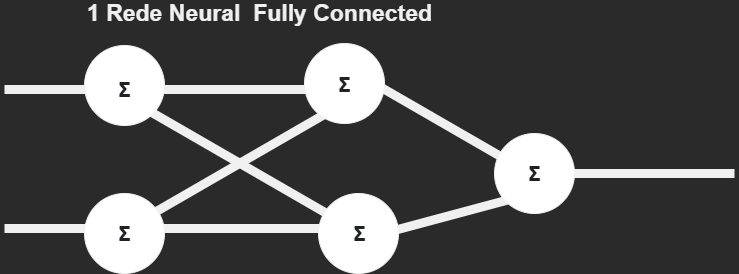
\includegraphics[width=7cm]{images/1_RN_FULLY CONNECTED.png}\break
    
\end{center}
\begin{center}
    
     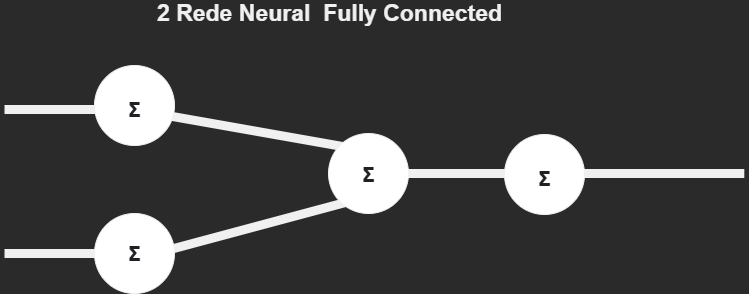
\includegraphics[width=7cm]{images/2_RN_FULLY CONNECTED.png}\break
\end{center}

    \end{itemize}
    

\end{itemize}




 
%
%%%%%%%%%%%%%%%%%%%%%%%%%%%%%%%%%%%%%%%%%%%%%%%%%%%%%%%%%%%%%%
%
\subsection{Pygame}\label{sec:ANN}

Pygame é um conjunto de plataforma cruzada de módulos Python que é usado para criar videogames.
Consiste em computação gráfica e bibliotecas de som projetadas para serem usadas com a linguagem de programação Python.
Pygame foi oficialmente escrito por Pete Shinners para substituir PySDL.
Pygame é adequado para criar aplicativos do lado do cliente que podem ser potencialmente agrupados em um executável autônomo.
O seu nome tem origem da junção de Py, proveniente de Python e Game, que significa Jogo, ou seja, Jogos em Python.
Gênero(s): Motor de jogo
Idioma(s): inglês
Licença: LGPL
Versão estável: 2.0.1 (24 de dezembro de 2009)
Linguagens de programação: Python, C, Cython, Linguagem assembly\cite{pygame_info_wikipedia}


\subsection{Python}\label{sec:ANN}
Python é uma linguagem de programação interpretada, orientada a objetos e de alto nível Tem ocupado o primeiro lugar no índice do TIOBE no ano de 2021.
O índice da comunidade de programação TIOBE é um indicador da popularidade das linguagens de programação, e pode ser usado como termômetro e um guia para tomada de decisão estratégica sobre qual linguagem de programação deve ser adotada ao iniciar a construção de um novo sistema de software.
As classificações são baseadas no número de engenheiros qualificados em todo o mundo, cursos e fornecedores terceirizados, motores de busca populares como Google, Bing, Yahoo, Wikipedia, Amazon, YouTube e Baidu são usados ​​para calcular as classificações.
O índice do TIOBE não trata da melhor linguagem e sim a mais popular entre os engenheiros e motores de busca da internet.
\cite{tiobe} Python e a extensa biblioteca padrão estão disponíveis em formato de código-fonte ou binário gratuitamente para todas as principais plataformas e podem ser distribuídos gratuitamente.. Foi lançada por Guido van Rossum em 1991
Criado Por: Guido van Rossum
Empresa matriz: Python Software Foundation\cite{python_info_wikipedia}.

\subsection{\textbf{Visão geral do NEAT}}\label{sec:ANN}
%
NEAT é um método desenvolvido por Kenneth O. Stanley para a evolução de redes neurais arbitrárias. NEAT-Python é uma implementação em Python pura do NEAT, sem dependências além da biblioteca padrão do Python.\\
São algoritmos baseados na biologia humana
os quais se utilizam de estrutura chamadas de neurônios 
agrupados para formar uma nova estrutura chamada de rede neural artificial
e esses neurônios são como variáveis para modelar um hiperplano,
que precisa ser modelado para encaixar numa equação a qual descreva seu problema.\\ 
Também devemos abordar sobre aprendizado, pois é por ele que o hiperplano é modelado,
citarei três maneiras de aprendizado porém focaremos na terceira e última, pois é o que dá base para neuroevolução e NEAT.\\
		
		
{\bfseries Aprendizado:}

\begin{itemize}

\item Aprendizado Supervisionado 
\item Aprendizado não-Supervisionado 
\item Aprendizado por Reforço:
\begin{itemize}
\item \emph{A aprendizagem por reforço lida com os conceitos de recompensas e
penalidades. O objetivo dessa modalidade é escolher um conjunto de ações que
maximize as recompensas}
\end{itemize}
\end{itemize}

%






